\documentclass[13pt,a4paper]{extarticle}
\usepackage[utf8]{inputenc}
\usepackage[utf8]{vietnam} %Bien dich duoc tieng Viet
\usepackage{amsmath,amsfonts,amssymb} %Font toan
\usepackage{type1cm}
\usepackage{graphicx}
\graphicspath{ {images/} }
\usepackage[unicode,hidelinks=true]{hyperref} %Tu dong tao bookmark
\usepackage{indentfirst} %Thut vao dau dong o tat ca cac doan
\usepackage{lscape}
\usepackage{csvsimple}
\usepackage{listings} %Dinh dang code
\usepackage{color} %Mau sac
\usepackage[left=2.5cm,right=1.5cm,top=1.5cm,bottom=1.5cm]{geometry} %Canh lề trái - phải - trên - dưới cho tài liệu
\definecolor{dkgreen}{rgb}{0,0.6,0}
\definecolor{gray}{rgb}{0.5,0.5,0.5}
\definecolor{mauve}{rgb}{0.58,0,0.82}

\lstset{frame=tb,
  language=C,
  aboveskip=3mm,
  belowskip=3mm,
  showstringspaces=false,
  columns=flexible,
  basicstyle={\small\ttfamily},
  numbers=left,
  numberstyle=\tiny\color{gray},
  keywordstyle=\color{blue},
  commentstyle=\color{dkgreen},
  stringstyle=\color{mauve},
  breaklines=true,
  captionpos=t,
  breakatwhitespace=true,
  tabsize=2
}
\begin{document}
\title{\textbf{NỘI DUNG CHUẨN BỊ BUỔI 1}}
\author{Sinh viên thực hiện: Thi Minh Nhựt\thanks{\textsf{Email thiminhnhut@gmail.com}}}
\date{Ngày 21 tháng 04 năm 2016}
\maketitle
\section{Phần cứng}
Vi điều khiển \verb|Arduino Pro Mini|; cảm biến siêu âm \verb|HY-SRF05|; màn hình hiển thị \verb|LCD 16x02| có kèm giao tiếp \verb|I2C|.
\section{Bộ cảm biến đo mực nước}
\begin{center}
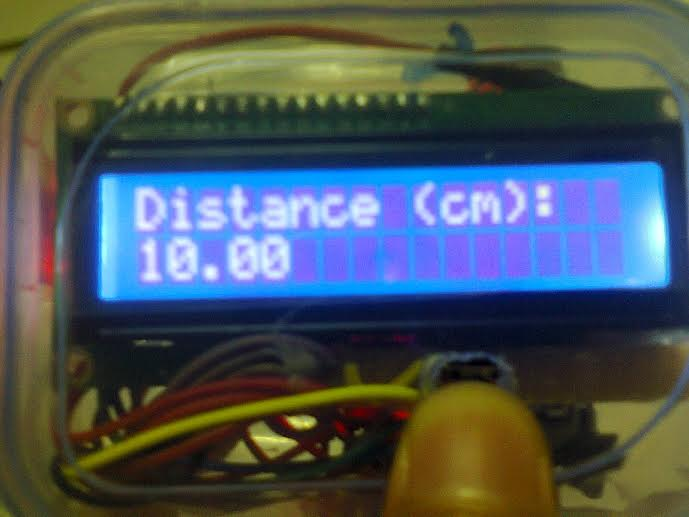
\includegraphics[scale=.3]{do-muc-nuoc-voi-cam-bien-sieu-am}
\end{center}
\section{Phần mềm}
\subsection{Cách tính khoảng cách với cảm biến siêu âm}
\lstinputlisting[language=C]{Distance_SRF.c}
\subsection{Hiển thị kết quả đo lên LCD}
Sử dụng thư viện \verb|LiquidCrystal_V1.2.1|\footnote{\textsf{https://bitbucket.org/fmalpartida/new-liquidcrystal/downloads}} viết cho \verb|Arduino|.
\section{Giải thuật sử lý số liệu đo}
\subsection{Giải thuật}
\begin{itemize}
\item Ta thực hiện $N$ lần đo được $N$ số liệu $A_i$ (tập $A$).
\item Thực hiện vòng lặp giảm dần các giá trị sau số $\delta _{j}$ theo các giá trị $$\delta _{max} = {50\%, 40\%, 30\%, 20\%, 10\%, 5\%}$$
\item Trong mỗi vòng lặp theo giá trị $A_i$:
\begin{itemize}
\item Gọi giá trị trung bình khi bỏ $A_i$ là $TBT_i$
\item So sánh: $|A_i - TBT_i| > TBT_i \times \delta_j$ thì bỏ $A_i$ ra khỏi tập $A$.
\end{itemize}
\item Sau cùng chỉ xuất giá trị trung bình $TB$ của các phần tử trong tập $A$ còn đang được xét sau khi thực hiện xong các vòng lặp trên.
\end{itemize}
\subsection{Chương trình}
\lstinputlisting[language=C]{giai-thuat.c}
\subsection{Kết quả}
Qua đo đạc thực tế với cảm biến siêu âm, em thu được bảng giá trị và áp dụng giải thuật trên được kết quả như trong bảng.
\begin{landscape}
\csvreader[tabular=|c|l|l|l|l|l|l|l|l|,
table head=\hline {}& Giá trị đo & Lọc$50\%$ &  Lọc $40\%$ & Lọc $30\%$ & Lọc $20\%$ & Lọc $10\%$ & Lọc $5\%$&  Trung bình\\\hline, late after line=\\\hline]%
{data1.csv}{}%
{\csvcoli& \csvcolii & \csvcoliii &\csvcoliv&\csvcolv&\csvcolvi&\csvcolvii&\csvcolviii&\csvcolix}
\end{landscape}
\begin{landscape}
\csvreader[tabular=|c|l|l|l|l|l|l|l|l|,
table head=\hline {}& Giá trị đo & Lọc$50\%$ &  Lọc $40\%$ & Lọc $30\%$ & Lọc $20\%$ & Lọc $10\%$ & Lọc $5\%$&  Trung bình\\\hline, late after line=\\\hline]%
{data2.csv}{}%
{\csvcoli& \csvcolii & \csvcoliii &\csvcoliv&\csvcolv&\csvcolvi&\csvcolvii&\csvcolviii&\csvcolix}
\end{landscape}
\section{Thêm tín năng}
Thêm tín năng giao tiếp giữa vi điều kiển và máy tính qua cổng nối tiếp RS232.

Lưu dữ liệu cảm biến đo được vào bộ nhớ ngoài.
\tableofcontents
\end{document}